% !TEX bibfile = ref.bib
\documentclass[11pt]{article}
\usepackage{latexsym}
\usepackage{amsmath,amssymb,amsthm}
\usepackage{epsfig}
\usepackage[right=0.8in, top=1in, bottom=1.2in, left=0.8in]{geometry}
\usepackage{setspace}\usepackage{graphicx} %插入图片的宏包
\usepackage{float} %设置图片浮动位置的宏包
\usepackage{subfigure} %插入多图时用子图显示的宏包
\usepackage{algorithm}
\usepackage{algorithmic}
\renewcommand{\algorithmicrequire}{\textbf{Input:}}  % Use Input in the format of Algorithm
\renewcommand{\algorithmicensure}{\textbf{Output:}} % Use Output in the format of Algorithm
\usepackage{listings}
\usepackage{ctex}

% 用来设置附录中代码的样式

\lstset{
    basicstyle          =   \sffamily,          % 基本代码风格
    keywordstyle        =   \bfseries,          % 关键字风格
    commentstyle        =   \rmfamily\itshape,  % 注释的风格,斜体
    stringstyle         =   \ttfamily,  % 字符串风格
    flexiblecolumns,                % 别问为什么,加上这个
    numbers             =   left,   % 行号的位置在左边
    showspaces          =   false,  % 是否显示空格,显示了有点乱,所以不现实了
    numberstyle         =   \zihao{-5}\ttfamily,    % 行号的样式,小五号,tt等宽字体
    showstringspaces    =   false,
    captionpos          =   t,      % 这段代码的名字所呈现的位置,t指的是top上面
    frame               =   lrtb,   % 显示边框
}

\lstdefinestyle{Python}{
    language        =   Python, % 语言选Python
    basicstyle      =   \zihao{-5}\ttfamily,
    numberstyle     =   \zihao{-5}\ttfamily,
    keywordstyle    =   \color{blue},
    keywordstyle    =   [2] \color{teal},
    stringstyle     =   \color{magenta},
    commentstyle    =   \color{red}\ttfamily,
    breaklines      =   true,   % 自动换行,建议不要写太长的行
    columns         =   fixed,  % 如果不加这一句,字间距就不固定,很丑,必须加
    basewidth       =   0.5em,
}

\spacing{1.06}

\newcommand{\handout}[5]{
  \noindent
  \begin{center}
  \framebox{
    \vbox{\vspace{0.25cm}
      \hbox to 5.78in { {SE3352:\hspace{0.12cm}Algorithm Design} \hfill #2 }
      \vspace{0.48cm}
      \hbox to 5.78in { {\Large \hfill #5  \hfill} }
      \vspace{0.42cm}
      \hbox to 5.78in { {#3 \hfill #4} }\vspace{0.25cm}
    }
  }
  \end{center}
  \vspace*{4mm}
}
\newcommand{\lecture}[4]{\handout{#1}{#2}{#3}{Scribes:\hspace{0.08cm}#4}{Notes #1}}

\newtheorem{theorem}{Theorem}
\newtheorem{corollary}[theorem]{Corollary}
\newtheorem{lemma}[theorem]{Lemma}
\newtheorem{observation}[theorem]{Observation}
\newtheorem{example}[theorem]{Example}
\newtheorem{definition}[theorem]{Definition}
\newtheorem{claim}[theorem]{Claim}
\newtheorem{fact}[theorem]{Fact}
\newtheorem{assumption}[theorem]{Assumption}
\newcommand{\E}{\textbf{E}}
\newcommand{\var}{\text{var}}
\def\eps{\ensuremath\epsilon}
\begin{document}

\lecture{1 -- Clustering}{Nov 27, 2021}{Instructor:\hspace{0.08cm}\emph{Guoqiang Li}}{\emph{Haotian Wang, Yiyan Li}}


\section{Introduction}
Clustering can be considered the most important unsupervised learning problem; As every other problem of this kind, it deals with finding a structure in a collection of unlabeled data.
\begin{definition}
A cluster is a collection of objects which are “similar” between them and are “dissimilar” to the objects belonging to other clusters. Clustering is the algorithm that recognizes clusters from a given data set.
\end{definition}
Note that this is a very rough definition. Part of common application domains in which the clustering problem arises are as follows:
\begin{itemize}
\item \textbf{Multimedia Data Analysis:} Learning image or video representations without manual annotations. e.g. When using Streaming media platform, face clustering can recognize all the actors in any frame. \cite{wang2019linkage,xing2021learning}
\item \textbf{Responding to public health crises:} With the increasing number of samples, the manual clustering of COVID-19 data samples becomes time-consuming. Clustering helps classify medical datasets deterministically.\cite{COVID-19}
\item \textbf{Social Network Analysis:} Clustering provides an important understanding of the community structure in the network. Results can be used for customer segmentation and sending ads. Put it in a formal way, \textbf{clustering groups the nodes of the graph into clusters}, taking into account the edge structure of the graph in such a way that there are several edges within each cluster and very few between clusters. \cite{community}
\item \textbf{Intermediate Step for other fundamental data mining problems:} Clustering can be considered as a form of data summarization. Many clustering methods are closely related to dimensionality reduction methods. Such methods can be considered a form of data summarization.
\item \textbf{Intelligent Transportation:} Under \textbf{the online scenario}, data is in the form of streams, i.e., the whole dataset could not be accessed at the same time. In future intelligent transportation, low-latency online vehicle tracking is essential and can be solved by online clustering.\cite{luna2021online}

\end{itemize}

\par Today we'll start from the naive K-means clustering and improve the algorithm step by step. The lecture has X main topics that we'll go through, i.e. TODO AL LAST!!

\section{Problem Description}
\begin{definition}
\textbf{Cluster centroid} is the middle of a cluster. A centroid is a vector that contains one number for each variable, where each number is the mean of a variable for the observations in that cluster. The centroid can be thought of as the multi-dimensional average of the cluster.
\end{definition}
\par The k-means clustering problem is one of the oldest and most important questions in all of computational geometry. Given an integer $k$ and a set of $n$ data points in $\mathbb{R}^{d}$, the goal of this problem is to choose $k$ centers so as to minimize the total squared distance between each point and its closest center.\cite{kmeanspp}
\par There are several kinds of k-means algorithms among which the most common algorithm , also called naive k-means algorithm, was first proposed by Stuart Lloyd\cite{Least-squares-quantization-in-PCM} of Bell Labs in 1957.
\par For a k-means problem, we are given an integer $k$ and a set of data vector ($x_1, x_2, x_3 \dots x_n$) in $d$-dimension. And we need to choose $k$ centroids to partition the $n$ vectors into $k$ types $T$ ($T_1, T_2 \dots T_k$) with the minimum within-cluster sum of squares ($WCSS$)
$$\mathcal{WCSS} = \arg \min \sum_{i=1}^{k} \sum_{x \in S_i } {\left\lVert x - c _i \right\rVert }^2  $$
\par where $\mu_i$ is the mean of vector in set $S_i$.

\begin{lemma}
  Let $S$ be a set of points with its mean to be $\mu$, and let $c$ to be and arbitrary point.Then $\sum_{x \in S}{\left\lVert x - c\right\rVert}^2 = \sum_{x \in S}{\left\lVert x - \mu\right\rVert}^2 + \left\lvert S \right\rvert \cdot {\left\lVert z - \mu\right\rVert}^2 $
\end{lemma}
\par So we minimize the function only when $c_i=\mu_i$
\begin{equation*}
  \begin{split}
    \mathcal{WCSS} & = \arg \min \sum_{i=1}^{k} \sum_{x \in S_i } {\left\lVert x - c _i \right\rVert }^2 \\
    & = \arg \min \sum_{i=1}^{k} (\sum_{x \in S_i} {\left\lVert x - \mu_i\right\rVert}^2 + \left\lvert S_i \right\rvert \cdot {\left\lVert c_i - \mu_i\right\rVert}^2) \\
    & = \arg \min \sum_{i=1}^{k} {\left\lvert S_i \right\rvert }\cdot Var S_i \\
    & = \arg \min \sum_{i=1}^{k} \frac{1}{2\cdot\left\lvert S_i\right\rvert } \sum_{x,y \in S_i} {\left\lVert x_i - y_i\right\rVert }^2
  \end{split}
\end{equation*}


\section{Algorithms}
% origin K means
\subsection{The K-means algorithm}
\subsubsection{Algorithm Details}
The k-means algorithm is a simple and fast algorithm for this problem, although it offers no approximation guarantees at all.
It iteratively calculates the sum of distance within a cluster and updates the partition.The details are as follows.\cite{k-means}
\begin{enumerate}
  \item Arbitrarily choose and initial $k$ centers $\mathcal{C} = \{c_1, c_2 \dots c_k\}$
  \item For each $i \in \{1, 2 \dots k\}$, set the cluster $C_i$ to be the set of points that are closer to $c_i$ than they are to $c_j$ for all $j \neq i$
  \item For each $i \in \{1, 2 \dots k\}$, set $c_i$ to be the center of all points in $C_i$ 
  \item Repeat Step 2 and Step 3 until $\mathcal{C}$ no longer changes.
\end{enumerate}
\begin{algorithm}
  \caption{K-means}
  \label{k-means}
  \begin{algorithmic}
    \REQUIRE {k: number of output cluster; Data: input data}
    \ENSURE {$\mathcal{S}$ : set of all clusters $S_i$}
    \STATE Arbitrarily initialize k centroids $C=\{c_1, c_2 \dots c_k\}$ 
    \REPEAT
      \FOR {each point $x$ in Data $S$}
      \FOR {$i = 0 \rightarrow k$}
      \FOR {$j = 0 \rightarrow k$}
      \STATE {set x to be a member of cluster $S_i$ where ${\left\lVert x-c_i\right\rVert }^2 < {\left\lVert x-c_j\right\rVert }^2$}
      \ENDFOR
      \ENDFOR
      \ENDFOR
      \FOR {$i = 0 \rightarrow k$}
      \STATE {$c_i \leftarrow \frac{1}{\left\lvert S_i\right\rvert } \sum_{x \in S_i} x$}
      \STATE {set $c_i$ to be the centroid of all points in  cluster $S_i$}
      \ENDFOR
    \UNTIL{$S$ stays unchanaged}
    \ENSURE {$\mathcal{S}$ : set of all clusters $S_i$}
  \end{algorithmic}
\end{algorithm}

\begin{proof}
  Let $x_1, x_2 \dots x_n$ be n vectors in $\mathbb{R}^{d}$, then $f(x) = \sum_{i=1}^{n} {\left\lVert x_i - x\right\rVert}^2 $ gets its minimum iff. $x = \frac{1}{n} \sum_{i=1}^{n}x_i$
  \begin{equation*}
    \begin{split}
      \frac{d f(x)}{d x} &=  \frac{d \sum_{i=1}^{n} {\left\lVert x_i - x\right\rVert}^2}{d x} \\
      & = -2\sum_{i=1}^{n} (x_i - x) \\
      & = 0 \\
      x & = \frac{1}{n} \sum_{i=1}^{n}x_i
    \end{split}
  \end{equation*}
  
  \par $x = \frac{1}{n} \sum_{i=1}^{n}x_i$ is a stationary point of this function. Owing that it is a strictly convex function, the stationary point is alse the only minimun point of that function. 
  So the function gets its minimum at $x = \frac{1}{n} \sum_{i=1}^{n}x_i$.
  \end{proof}
  \begin{proof}
    Updated value $f(x'')$ is strictly less than the original $f(x')$ where  $x'' = \frac{1}{n} \sum_{i=1}^{n}x_i$.
  \par As described above, each centroid is updated to the center of all points in cluster $C_i$. 
  That is to say, once the centroid of one cluster changed from $x'$ to  $x'' = \frac{1}{n} \sum_{i=1}^{n}x_i$, the function gets its minimum in this iteration at $x''$ and $f(x'')<f(x')$.
  \end{proof}
  \subsubsection{DrawBack}
  The naive K-means algorithm do great work for the simplicity and efficiency, but it also has drawbacks. In the caes of initializing $k$ centroids using naive K-means algorithm (usually Lloyd's algorithm), we use randomization.
  The initial $k$ centroid are picked in the range of data set randomly. However, this initialization strategy could result in initialization sensitivity. The final formed clusters could be affected greatly by the initial picked centroids.
  \par Here are a few figures showing the potential:
\begin{figure}[H] %H为当前位置,!htb为忽略美学标准,htbp为浮动图形
  \centering %图片居中
  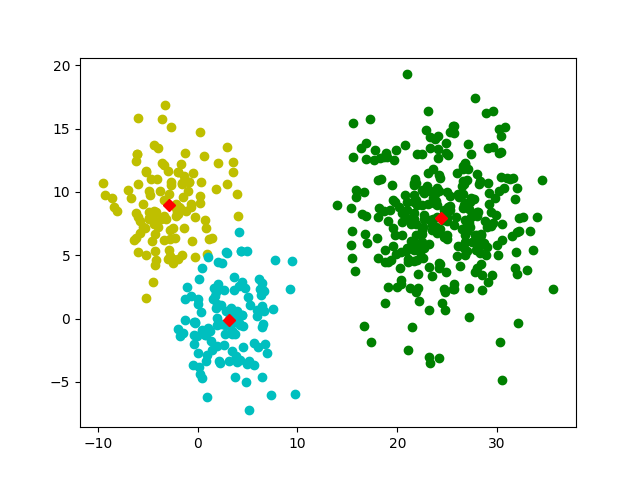
\includegraphics[width=0.5\textwidth]{goodCluster.png} %插入图片,[]中设置图片大小,{}中是图片文件名
  \caption{Good Cluster} %最终文档中希望显示的图片标题
  \label{Fig.GoodCluster} %用于文内引用的标签
\end{figure}
\begin{figure}[H] %H为当前位置,!htb为忽略美学标准,htbp为浮动图形
  \centering %图片居中
  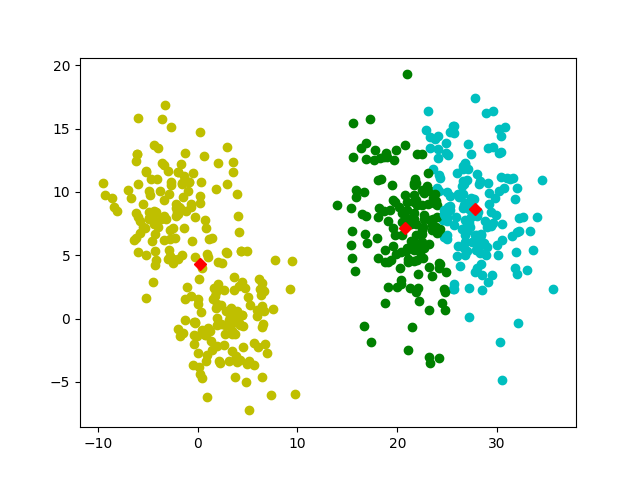
\includegraphics[width=0.5\textwidth]{badCluster.png} %插入图片,[]中设置图片大小,{}中是图片文件名
  \caption{Bad Cluster} %最终文档中希望显示的图片标题
  \label{Fig.BadCluster} %用于文内引用的标签
\end{figure}
\par In the above images, the final formed clusters are pretty different. The good cluster's\cite{Fig.GoodCluster} initial $k$-centroids are initialized in different clusters, leading to a good result. While the other one's\cite{Fig.BadCluster} initial centroids were unfortunately initialized in the same cluster and got a result which was not as expected.

% sum of optimiazation
\subsection{Optimization of K-means}
In last several decades, there has been significant work on improving Lloyd’s algorithm both in terms of reducing MSE and running time. The follow up
work on Lloyd’s algorithm can be broadly divided into three categories:
\begin{enumerate}
\item Better seed selection
\item Selecting ideal value for number of clusters
\item Bounds on data point to cluster centroid distance
\end{enumerate}
Next, we will introduce some typical work in these categories. Section 3.3 introduces K means++ for seed selection, section 3.4 and 3.5 helps bound on data point to cluster centroid distance and section 3.6 introduces several typical methods to select ideal value for number of clusters briefly. Let's begin.


% kmeans ++
\subsection{The K-means++ algorithm}
The K-means++ algorithm was proposed by David Arthur and Sergei Vassilvitskii in 2006, which outperforms K-means in terms of both accuracy and speed \cite{kmeanspp}.
\par The K-means++ algorithm uses totally a different way to initialize the $k$ centroids. Rather than uniformly randomly pick point in the range of all points, it uses special to make the $k$ centroids as far away from each other as possible.
And the updated algorithm does exactly the same in the iteration steps. The algorithm goes as follows:
\begin{enumerate}
  \item Pick the first centroid $c_1$ randomly from the dataset $S$
  \item Compute the distance of all points in the dataset from centroid $c_1$. The distance of a point $x$ could be calculated by $$ Dist(x, c_i) = {\left\lVert x-c_i\right\rVert } $$
  \item Take a new centroid $c_i$, choosing $x_j \in $ from all points with probability $p_j$ $$p_j = \frac{Dist^2(x_j)}{\sum_{x_j \in S} Dist^2(x_j)} $$
  \item Repeat the above steps until $k$ cetnroids are found
  \item Iteration steps are exactly the same as navie K-means algorithm
\end{enumerate}
\par k-means++ consistently outperformed k-means, both by achieving a lower potential value,
in some cases by several orders of magnitude, and also by completing faster. With the synthetic
examples, the k-means method does not perform well, because the random seeding will inevitably
merge clusters together, and the algorithm will never be able to split them apart. The careful
seeding method of k-means++ avoids this problem altogether, and it almost always attains the
optimal results on the synthetic datasets.\cite{kmeanspp}

% opt 2
\subsection{Reduce cost of single iteration}
In both K-means and K-means$++$ algorithm, if there are $n$ data points in $\mathbb{R}^ d$ space and $k$ clusters for partition, each iteration involves $n * k$ distance computations, which would significantly slow down algorithm. One contribution from Siddhesh Khandelwal\cite{Faster} helps reduce this cost to $n * k^{\prime}$ ($k^{\prime} << k$) by generating candidate cluster list (CCL) of size $k^{\prime}$ for each data point. We'll show how this heuristic works in detail.
\subsubsection{Inspiration}
The optimization is based on the observation that across all iterations of K-means or K-means$++$, a data point changes its membership only among a small subset of clusters. The heuristic considers only a subset of \textbf{nearby cluster as candidates} for deciding membership for a data point. This heuristic has advantage of speeding up K-means and K-means$++$ clustering with marginal increase in loss functuion(MSE in our case). Note that the optimization can be applied in any algorithm to solve K-means problem with steps to caculate distance between points and centers, acting as augmentation.
\subsubsection{Augmentation target}
Let $A$ be any variant algorithm of K-means problem and $B$ be the same variant augmented with this geuristic. Let $T$ be the time required for $A$ to converge to MSE value of $E$. Let $T^{\prime}$ be the time required for $B$ to converge to MSE value of $E^{\prime}$. Our target is:
\begin{itemize}
\item \textbf{For convergence time:} $T^{\prime} < T$
\item \textbf{For loss:} $E^{\prime} \le E \space $ or $ \space E^{\prime} \overset{marginally}{>} E$
\end{itemize}

\subsubsection{Augmentation detail}
\par We assume that $k^{\prime}$ is significantly smaller than $k$. We will show how to choose $k^{\prime}$ later.We build candidate cluster list (CCL) based on top $k^{\prime}$ nearest clusters to the data point after first iteration of K-means. \par

Consider a data point p1 and cluster centroids represented as $c_1$, $c_2$..., $c_k$. We assume that $k^{\prime}$ = 4, and $k^{\prime} << k $. After first iteration of K-means $c_5$, $c_6$, $c_8$, and $c_{11}$ are the top four closest centroids to $p_1$ in the increasing order of distance. This is the candidate cluster list for $p_1$. If we run K-means for second iteration, $p_1$ will compute distance to all k centroids. After second iteration, there are two possible cases:
\begin{enumerate}
\item The list do not change but only members'ranking changes.
\item Several members of the centroids in the previous list are replaced with other centroids which were not in the list.
\end{enumerate}
It seems that the augmentation makes no sense. But what makes this method succeed is \textbf{real world data rarely makes case 2 happen}. That is, the set of top few closest centroids for a data point \textbf{remains almost unchanged even though order among them might change}.
\subsubsection{Augmentation analysis}
Overhead analysis:
\begin{itemize}
\item \textbf{Computation overhead:} $O(nklog(k))$ for creating CCL at first. We have to compute the distance to each cluster's centroid for each point and sort them to create CCL. 
\item \textbf{Memory overhead:}$ O(nk^{\prime})$ to maintain CCL.
\end{itemize}
\par

% opt 3
\subsection{Avoid redundant computation}
In fact, the previous augmentation \cite{Faster} makes trade-off between loss function and running time. Still based on the observation of  unnecessary calculation in the process of iteration, Charles Elkan put forward a more strict method to avoid unnecessary computation.\cite{articleToBound} The key idea is to bound on data point to cluster centroid distance and use triangle inequality to avoid redundant computations of distance between data points and cluster centroids.
\subsubsection{Inspiration}
The accelerated algorithm applyies the triangle inequality in two different ways, and keeps track of lower and upper bounds for distances between points and cluster centroids. Its inspiration is based on the fact that most distance calculations in standard K-means are redundant. If a point is \textbf{far away from a centroid}, it is not necessary to calculate the exact distance between the point and the centroid in order to know that the point should not be assigned to this centroid. Conversely, \textbf{if a point is much closer to one center than to any other}, calculating exact distances is not necessary to know that the point should be assigned to the first center. 
\subsubsection{Augmentation target}
There are 3 properties the accelerated K-means algorithm should satisfy:
\begin{itemize}
\item \textbf{Start with any initial centers}, so that all existing initialization methods incuding original K-means and K-means++ can continue to be used.
\item \textbf{Correct results, } it always produces exactly the same final centers as the standard  algorithm.
\item \textbf{Support any black-box distance metric,} so it should not rely for example on optimizations specific to Euclidean distance.
\end{itemize} \par
Obviously, It's more strict than previous method. This stronger properties mean that more basic K-means algorithms are able to install this augmentation. e.g., heuristics for merging or splitting centers can be used together with the new algorithm.(e.g. ISODATA, which not memtioned in our note)

\subsubsection{Preliminary results}
The algorithm firstly find the only black box property of any distance metrics.That is: for any 3 points $x, y, z$, satisfy  triangle inequality:
$$d(x,z) \le d(x, y) + d(y, z)$$ in which $d()$ means distance function. Let x be a point and let b and c be centers, we need to know that $d(x, c) \ge d(x, b)$ in order to avoid calculating $d(x, c)$. Now I'd like to introduce 2 Lemma.
\begin{lemma}
Let x be a point and let b and c be centers. If $d(b, c) \ge 2d(x,b)$ then $d(x,c) \ge d(x,b)$.
\end{lemma}
\begin{proof}
Use  triangle inequality, $d(b,c) - d(x,b)\le d(x,c)$. Use "if" in lemma, we can get the conclusion.
\end{proof}
\begin{lemma}
Let x be a point and let b and c be centers.$d(x,c) \ge max(0, d(x,b)-d(b,c))$.
\end{lemma}
\begin{proof}
Use triangle inequality, with $d(x,c) \ge 0$, easily get lemma 5.
\end{proof}

Let x be any data point, let c be the center to which is currently assigned, let s become any other center. So with the lemma, we can assert that:
\begin{claim}
if $\frac{1}{2}d(c, s) \ge d(x,c)$ then $d(x, s) \ge d(x, c)$, and we don't need to compute $d(x,s)$. (Proved by lemma)
\end{claim}
\begin{claim}
Suppose that we don't know $d(x,c)$ exactly, and we do know an upper bound u such that $u \ge d(x,c)$: For any other possible choice, we only need to compute $d(x, c), d(x, s)$ iff $u > \frac{1}{2}d(c, s)$ .(Proved by claim)
\end{claim}
\begin{claim}
Suppose that $u \le \frac{1}{2}d(c, s)$ for any possible s, all distance calculations for x can be avoided. (Proved by claim)
\end{claim}

Next, Let x be any data point, let c be any center, let s become previous version of smae center. Suppose that in the previous iteration we knew a lower bound g such that $d(x, s) \ge g$. Then we can infer a lower bound h for current iteration:
$$
d(x, c) \ge max\{0, d(x,s)-d(s,c)\} \ge max\{0, g-d(s,c)\} = h
$$
This can be easily proved by lemma 2. So we can assert that:
\begin{claim}
If center moved a small distance$(d(s,c) is small)$, the lower bound only make a small move.
\end{claim}

\subsubsection{Augmentation detail}
In practical application, as the centers are converging to their final positions, the vast majority of the data points have the same closest center from one stage to the next. A good algorithm would exploit this coherence to improve running time. We use $u(x)$ to represent upper bound of distance between a given point $x$ and its currently assigned center $c$. $l(x,c^{\prime})$ is the lower bound on the distance between x and some other center $c^{\prime}$. If $u(x) \le l(x,c^{\prime}) $, we don't need to calculate $d(x,c), d(x, c^{\prime})$. \par
Initially, we set $l(x,c)=0$ for each point x and center c. Then assign each x to its closest initial center, using Lemma 1 to firstly reduce redundant distance computations. Each time $d(x,c)$ is computed, set $l(x,c)=d(x,c)$. At last, set upper bounds $u(x) = min_c(d(x,c))$. Then repeate this until convergence.(Each time $d(x,c)$ is calculated, we update $l(x,c)$. Similarly $u(x)$ when computing $d(x,c(x))$.)

\begin{enumerate}
\item For all centers c and $c^{\prime}$, compute $d(c, c^{\prime})$. Set $s(c) = \frac{1}{2}min_{c \ne c^{\prime}}d(c,c^{\prime})$.
\item Identify all points x such that $u(x) \le s(c(x))$. (Refer to claim 8)
\item For each pair of remaining x and c, which satisfy: i) $c \ne c(x)$ and ii) $u(x) > l(x,c)$(obviously) and iii) $u(x) > \frac{1}{2}d(c(x), c)(Claim 7)$: 
\begin{enumerate}
\item If $r(x) = true$, compute $d(x,c(x))$ and assign $r(x)=false$. Otherwise, $d(x,c(x)) = u(x).$ (We don't have to update according to Claim 9)
\item  If $d(x,c(x))> l(x,c)$ or $d(x,c(x)) > \frac{1}{2}d(c(x), c)$, then compute $d(x,c)$ and decide if swap c for x. (Claim 7)
\end{enumerate}
\item For each center c, compute centroid, store in m(c).
\item For each  pair of x and c, set $l(x,c) = max(l(x,c) - d(c,m(c)), 0)$
\item For each point x, set $u(x) = u(x) + d(m(c(x)), c(x))$
\item For each point x, set $r(x) = True$
\item Really replace c by m(c)
\end{enumerate}

Logically, step (2) is redundant because its effect is achieved by condition 3(iii). Computationally, step (2) is benefificial in real experiment because reduce x's size for later steps. And note that u(x) and c(x) may change during the execution of step (3), so we can't discard condition 3(iii).\par
The most significant part is step (3), we use many strictions to avoid redundant computations. In 3(a) step, we only compute $d(x,c(x))$ for at most one time. Just when in pervious step (7) r(x) is set to True, we update  $d(x,c(x))$, or else we use u(x) to replace. Why step 3's strictions are effcient is that at the start of each iteration, the upper bounds and lower bounds for x are tight enough. If at $j^{th}$ iteration is tight, it'll be tight at $(j+1)^{th}$ iteration, because the location of most centers changes only slightly, and hence the bounds change only slightly. \par

\subsubsection{Augmentation analysis}
Compared to original algorithm, in 6 typical benchmark, using this optimazation speeds up algorithms from $ 11.3 \times$ to $  351 \times$.

% Opt 4
\subsection{Choose a proper K}
How to evaluate goodness of clustering for various potential values of number of clusters? We will introduce several common methods.\cite{datamining,inproceedings,articleToBound,doi:10.1243/095440605X8298} Let's review our optimization. We speed up the algorithm with either lenient or strict conditions and seed the initial K center properly. But still exists the only hyper-parameter we don't know how to tune. So let's begin. \par


\subsubsection{Use a range of set}
We choose a set of K and compare their performance. In this set, we need to choose k significantly smaller than the number of objects in the data sets and let it be resonably large.

\subsubsection{statistical measures}
There are several statistical measures available for selecting K. These measures are often applied in combination with probabilistic clustering approaches.
They are calculated with certain assumptions about the underlying distribution of the data. The Bayesian information criterion is calculated on data sets which are constructed by a set of \textbf{Gaussian distributions}. Monte Carlo techniques, which are associated with the null hypothesis, are used for assessing the clustering results and also for determining the number of clusters.

\subsubsection{visualization}
Visual verification is applied widely because of its simplicity and explanation possibilities. In my own practice, I usually use PCA or other methods to draw points on a planar graph to check how many clusters exist in Machine Learning course's project. But it has many restrictions. e.g. The application of
visualization techniques implies a data distribution continuity in the expected clusters. In fact, Visual examples are often used to illustrate the drawbacks of an algorithm. \par

\subsubsection{Determined in a later processing step}
When K-means clustering is used as a pre-processing tool, the number of clusters is determined by the specific requirements of the main processing algorithm. No attention is paid to the effect of the clustering results on the performance of this algorithm. In such applications, the K-means algorithm is employed just as a black box without validation of the clustering result. \par

\section{Key properties}
K means problem is an NP Hard problem, and two teams have proved them using 3-SAT and Exact Cover by 3-Sets respectively.\cite{npc-prove,Vattani_thehardness} Next, I'll try to describe the reduction from 3-SAT to k-means since NP-Complete problem is an inescapable topic in algorithm course. But I'll only describe informally.
\subsection{Reduction from 3-SAT to K-means}
Let {F} be the given planar 3-SAT instance with n variables and m clauses. We construct an instance I of planar k-means corresponding to F. Properties of layout I are listed below:
\begin{enumerate}
\item Each variable $x_i$ corresponds to a simple circuit $s_i$ in the plane and each circuit has an even number Q of vertices. Each vertex on such a circuit have M copies of a point. Note that M and Q will be stricted below. Now we can partiution
\item b
\item cc
\end{enumerate}


\section{Application}
In real world, K-means are widely used in clustering for its simplicity and effcient. Its core concept is extremely easy to understand and the updated version algorithm itself only cost a few iterations to output pretty good results. And here are a few applications of K-means algorithm in real life.
\subsection{Customer Segmentation}
The segmentation of the customers’ base allows operators to better serve customers and target advertising precisely to them\cite{Bcil2012PrepaidTC}.
The concept of segmentation relies on the high probability of persons grouped into segments based on common demands and behaviours to have a similar response to marketing strategies.
\par And the concept of segmentation coincides with that of clustering. A company can run K-means analysis base on customers' consumption habits, browsing histories, financial conditions and many other features to precisely partition their customers into different clusters so that they can implement different strategies.\cite{Bcil2012PrepaidTC}
\subsection{Optimization of Truck-Drone Delivery Netword}
The K-means algorithm is used to optimize truck-drone in tandem delivery network. One of the objectives is to investigate the time, energy, and costs associated to a truck-drone delivery network compared to standalone truck or drone. 
\par In 2016, Sergio Ferr{\'a}ndez, Timothy Harbison, Troy Weber, Robert H. Sturges and Robert Rich proposed a method\cite{Ferrndez2016OptimizationOA}, optimizing the delivery netword of drone powerd by K-means algorithm to find the appropriate launch locations with the  minimum cost.  The optimal solution is determined by finding the minimum cost associated to the parabolic convex cost function.
\subsection{Document Classification}
Clustering documents in multiple categories based on tags, topics, and the content of the document is a very standard classification problem and k-means is a highly suitable algorithm for this purpose.\cite{kmeansapplication}
\par All we need to do is to pre-processing the documents, representing each of them as a high-dimension vector and using term frequency to identify commonly used terms that help classify the document.
The document vectors are then treated as input of K-means algorithm to help identify similarities in document groups.\cite{Jacob2016ImprovedCO}

\subsection{Research based on COVID-19 Dataset}
Now we'll present a k-means clustering-based COVID-19 analysis to determine the clusters according to the health care quality of the countries. In fact we don't think this research meaningful, but just refer to their way to use K-Means in application.\cite{zubair2020efficient} \par
The team uses we use Principal Component Analysis (PCA)  whiledetermining the centroids.
\begin{figure}[H] %H为当前位置,!htb为忽略美学标准,htbp为浮动图形
  \centering %图片居中
  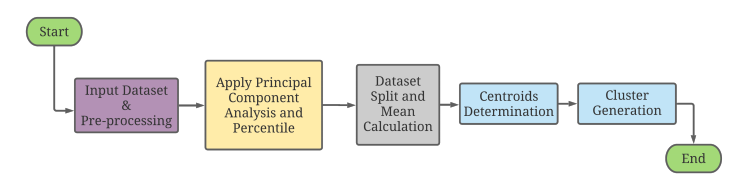
\includegraphics[width=0.5\textwidth]{COVID19.png} %插入图片,[]中设置图片大小,{}中是图片文件名
  \caption{Flowchart of centroids deciding} %最终文档中希望显示的图片标题
  \label{Fig.centroids} %用于文内引用的标签
\end{figure}
With this method to decide on centroids, the author argues that their method uses much less iterations and execution time for convergence. Compared with existing K-means++, their algorithm's performance is constant and faster. \par
But to be honest, we have to argue that their research just used K-means to generate clusters at last. In fact, after PCA, we can clearly observer that there are 3 kinds of COVID-19 situations over the world.(which fits our impression) What K-means does just verifies countries in detail. That is, without enough knowledge of dataset, we have to decide on cluster number with other methods. After that, K-means will generate clusters for us finally. That's what this article implies.


\section{Median Trick}
So far, we have an algorithm $A$ which estimates in correct range of $\eps$ with probability $\ge 0.9$. Our new algorithm $A^{\ast}$ will output in range of $\eps$ with probability $1-\delta$.
Algorithm:
\begin{itemize}
\item Repeat $A$ for $m=O(log (1/\delta))$ times
\item Take median of all the $m$ answers.
\end{itemize}

To prove the correctness, we'll use Chernoff/Hoeffding bounds.

\begin{definition}
[Chernoff/Hoeffding Bound]
Let $X_{1}$, $X_{2}$, $\ldots$, $X_{m}$ be independent random variables $\in \{0,1\}$,
$\mu = E[\Sigma_{i} X_{i}], \eps \in [0,1]$.
Then $Pr[|\Sigma_{i} X_{i}-\mu| > \eps\mu] \leq 2e^{-\eps^{2}\mu/3}$
\end{definition}

Define $X_{i} = 1$ iff the $i^{th}$ answer of $A$ is correct (i.e. estimated value of $A$ lies in correct range).

\begin{claim}
$E[X_{i}] = 0.9$, and $E[\mu] = 0.9m$
\end{claim}

\begin{proof}
Since A is correct with probability 0.9, $E[X_{i}] = 0.9$. And $E[\mu] = 0.9m$ due to linearity of expectation.
\end{proof}

\begin{claim}
New algorithm $A^{\ast}$ is correct when $\Sigma_{i} X_{i} > 0.5m$
\end{claim}

\begin{proof}
Since we are considering median value to be our answer, if more than half the trials of A are correct, algorithm $A^{\ast}$ is also correct.
\end{proof}

\begin{claim}
To prove, $Pr[\Sigma_{i} X_{i} \ge 0.5m] \ge 1-\delta$ or $Pr[\Sigma_{i} X_{i} < 0.5m] < \delta$
\end{claim}

\begin{proof}
\begin{equation}
\begin{split}
Pr[\Sigma_{i} X_{i} < 0.5m] & = Pr[\Sigma_{i} X_{i} - 0.9m < -0.4m]\\
& \le Pr[|\Sigma_{i} X_{i} - \mu| > 0.4m]\\
& = Pr[|\Sigma X_{i} - \mu| > 0.4/0.9 \mu]
\end{split}
\end{equation}
Using Chernoff bound,
\begin{equation}
\begin{split}
& \leq e^{-c*0.9m}\\
& < \delta
\end{split}
\end{equation}
Above equation holds for $m = O(log(1/\delta))$
\end{proof}

\section{Distinct Elements}
Given, a stream of size $m$ containing numbers from $[n]$, we have to approximate the number of elements with non-zero frequency. To calculate the exact value the space required:

\begin{itemize}
\item $O(n)$ bits. (maintain a vector of length n).
\item $O(m \log (n))$ bits. (save m numbers, each taking $log(n)$ bits).
\end{itemize}

Since, this complexity is not feasible as $m$,$n$ can be very large, we'll look at algorithm for approximating the distinct count value.

\subsubsection{Hash Function}
\begin{itemize}
\item $h : [n] \rightarrow [0,1]$
\item $h(i)$ is uniformly distributed in $[0,1]$.
\end{itemize}

\subsection{Algorithm [Flajolet-Martin 1985]}
We maintain a variable $z$.
\begin{enumerate}
\item Initialize $z = 1$.
\item Whenever $i$ is encountered: $z = \min{(z,h(i))}$
\item When done, output $1/z -1$.
\end{enumerate}

Now, we'll prove the algorithm works in a similar fashion followed in previous lecture.
Let $d$ be number of distinct elements.

\begin{claim}
$E[z] = d+1$
\end{claim}

\begin{proof}
$z$ is the minimum of $d$ random numbers in $[0,1]$. Pick another random number $a \in [0,1]$. The probability $a<z$:
\begin{enumerate}
\item exactly z
\item probability it's smallest among $d+1$ reals : $1/(d+1)$
\end{enumerate}
Equating these two, one can prove the claim.
\end{proof}

\begin{claim}
$\text{var}[z] \leq 2/d^{2}$
\end{claim}

\begin{proof}
It can be done in a similar fashion described in previous lecture.
\end{proof}

\subsubsection{$(1+\eps)$ approximation Algorithm }
We can take $Z = (z_{1} + z_{2} + ... z_{k})/k$ for independent $z_{1}, ... z_{k}$

\subsection{Alternate Algorithm: Bottom-k}
Instead of just use the minimum value of hash function for $i$ inputs, we'll maintain the $k$ smallest hashes seen.
\begin{enumerate}
\item Initialize $(z_{1}, z_{2},...z_{k}) = 1$.
\item Keep $k$ smallest hashes seen, s.t. $z_{1}\leq z_{2}\leq...z_{k}$
\item When done, output $\hat{d} = k/z_{k}$
\end{enumerate}

\begin{claim}
The following claims are stated:
\begin{itemize}
\item $Pr[\hat{d} > (1 + \eps)d] \leq 0.05$
\item $Pr[\hat{d} < (1 - \eps)d] \leq 0.05$
\item Overall probability that $\hat{d}$ outside range is at most 0.1
\end{itemize}
\end{claim}

\begin{proof}
To compute $Pr[\hat{d} > (1+\eps)d]$:
\begin{itemize}
\item Define $X_{i} = 1$ iff $h(i) < \dfrac{k}{(1+\eps)d}$
\item Then $\hat{d} > (1+\eps)d$ iff $\Sigma_{i} X_{i} > k$
\item if $\Sigma_{i} X_{i} > k$\\
  $\iff \exists$ at least $k$ numbers for which $h(i) < \dfrac{k}{(1+\eps)d}$\\
    \begin{equation}
      \iff z_{k} < \dfrac{k}{(1+\eps)d}
      \iff \dfrac{k}{z_{k}} > (1+\eps)d
      \iff \hat{d} > (1+\eps)d
    \end{equation}
\item
  $E[X_{i}] = \dfrac{k}{(1+\eps)d}$\\
  $E[\Sigma_{i} X_{i}] = d E[X_{i}] = \dfrac{k}{1 + \eps}$\\
  $\text{var}[\Sigma_{i} X_{i}] = d \text{var}[X_{i}] \leq dE[X_{1}^{2}] \leq  \dfrac{k}{1+\eps} \leq k$\\
  (Since $X_{1} \in \{0,1\}$, $E[X_{1}^{2}] = E[X_{i}]$)
\item By Chebyshev:
    $Pr[|\Sigma X_{i} - \dfrac{k}{1+\eps}| > \sqrt{20k}] \leq 0.05 \implies Pr[\Sigma X_{i} > \dfrac{k}{1+\eps} + \sqrt{20k}] \leq 0.05 $\\
    \begin{itemize}
    \item
      (For $\eps < 1/2$ and $k=c/\eps^{2}$)\\
      $\dfrac{k}{1+\eps} + \sqrt{20k} \leq k(1-\eps+\eps^{2}) + \sqrt{20k}$ (Taylor Series Expansion)\\
      $ \leq k - k\eps/2 + 5\sqrt{c}/\eps$
      $ = k - c / 2\eps + 5\sqrt{c}/\eps$\\
      $ < k $ where $c > 100$
    \item
      Since $k > \dfrac{k}{1+\eps} + \sqrt{20k} $ in our case and $\Sigma X_{i}$ is monotonically increasing, $Pr[\Sigma X_{i} > k] \leq Pr[\Sigma X_{i} > \dfrac{k}{1+\eps} + \sqrt{20k}] \leq 0.05$

    \end{itemize}
\end{itemize}
\end{proof}

\subsection{Hash functions in stream}
The hash function we used has two practical issues: (1) the return value should be a real number. (2) how do we store it?

Discretization can solve the first issue. Instead of all the real numbers in $[0, 1]$, we use hash function with range $\{0, \frac{1}{M}, \frac{2}{M}, \frac{3}{M}, \ldots, 1\}$. For large $M \gg n^{3}$, the probability that $d \le n$ random numbers collide is at most $\frac{1}{n}$.

For the second issue, we use pairwise independent function instead of independent function.

\begin{definition}
$h: [n] \rightarrow \{1, 2, \ldots M\}$ is pairwise independent if for all $i \ne j$ and $a, b \in [M]$, $\text{Pr}[h(i)=a \land h(j)=b]=\frac{1}{M^2}$
\end{definition}

It works because in previous calculation, we only care about pairs. We defined $X_i=1$ iff $h(i)$ is small than a threshold, then we computed $\text{var}[\Sigma X_i] = E[(\Sigma X_i)^2] - E[(\Sigma X_i)^2] = E[X_1X_1 + X_1X_2 + \ldots]- E[(\Sigma X_i)^2]$. Notice that $E[X_iX_j]$ is the same for fully random $h$ and pairwise independent $h$.

\begin{example}
[Construct a pairwise independent hash]
Assume $M$ is a prime number (if not, we can always pick a larger $M$ that is a prime number). We pick $p, q \in \{0, 1, 2, \ldots M-1 \}$ and the hash function $h(i) = pi+q \mod M$. In this construction we only need $O(\log M) = O(\log n)$ space (to store $p, q, M$).
\end{example}

\begin{proof}
$h(i)=a, h(j)=b$ is equivalent to $pi+q \equiv a, pj+q \equiv b$. So $p(i-j) \equiv a-b$ and $p \equiv (a-b)(i-j)^{-1}, q \equiv a - pi$. Since $M$ is a prime number, the unique inverse implies that there is only one pair $(p, q)$ satisfies it. And the probability that pair is chosen is exactly $\frac{1}{M^2}$.
\end{proof}

\section{Impossibility Results}

We have used both approximation and randomization to solve the distinct counting problem with space much less than $\min{(m, n)}$. Now we are wondering: can we omit either approximation or randomization to achieve the same space efficiency? The answer is no.

\subsection{Deterministic Exact Won't Work}

First, we will show that there is no deterministic (no randomization) and exact (no approximation) way to solve it.

Suppose there do exists a deterministic and exact algorithm $A$ and an estimator function $R$ that use space $s \ll n, m$. That is, for a given integer stream, we first run the algorithm $A$ on the stream. As the stream goes $A$ will return middle memory steps, and we obtain the final memory state $\sigma$ after the stream ends. Then we apply $R$ on $\sigma$ to obtain our estimator $\hat{d}$. Since both $A$ and $R$ are deterministic and exact, $\hat{d}$ must equals to the distinct count for the stream.

We now build a binary representation $x$ of the stream with the following rules: (1) $x \in \{0, 1\}^{n}$, (2) $i$ in stream iff $x_i = 1$. For example, if 1, 3, 5, 6, 7 are in the stream and 2, 4 are not, $x$ will start with 1, 0, 1, 0, 1, 1, 1. Notice that each stream has a corresponding representation and streams containing different numbers have different representations.

\begin{claim}
We can recover the $x$ of the stream given the memory state $\sigma$
\end{claim}

\begin{proof}
Denote $d=R(\sigma)$ be the original estimator. Now we treat $\sigma$ as a middle snapshot of the memory and add integer $i$ as the next element of the stream. Now $A$ will return another memory state $\sigma'$, and $d'=R(\sigma)'$ will be our new estimator. If $d'=d$, $i$ must have appeared in the stream before since $A$ and $R$ are deterministic and exact. Similarly, if $d'>d$, $i$ must have not appeared in the stream before. Using this method with $i=1, 2, 3\ldots$ and we can recover the $x$.
\end{proof}

Since we can recover $x$ from $\sigma$, we can treat $\sigma$ as an encoding of a string $x$ of length $n$. But $\sigma$ has only $s \ll n$ bits! Furthermore, we can treat $A$, the function that produces $\sigma$, as a function with domain $\{0, 1\}^{n}$ and $\{0, 1\}^{s}$. We can see that $A$ must be injective because if $A(x)=A(x')=\sigma$, the recoverability implies $x=x'$.

Hence $s \ge n$. Which implies that there is no deterministic and exact algorithm $A$ and an estimator function $R$ that use space $s \ll n, m$.

\subsection{Deterministic Approx. Won't Either}

We can use the similar strategy to prove that deterministic approx. won't work. We pick $T \subset \{0, 1\}^{n}$ that satisfies the following conditions: (1) for all distinct $x, y \in T$, the number of digits $i$ that $y_i=1$ and $x_i=0$ should $\ge \frac{n}{6}$. (2) $|T| \ge 2^{\Omega(n)}$. Now we use algorithm $A$ to encode an input $x$ into $\sigma=A(x)$ and our estimator would be $\hat{d}=R(\sigma)$.

Now we want to recover $x$ based on $\sigma$, as what we have done in the last section. For a given $\sigma$ and any $y \in T$, we append $y$ to the stream and apply $A$ on it, and $A$ will return a memory state $\sigma'$. Using $\sigma'$ we have new estimator $\hat{d'}=R(\sigma')$.

\begin{claim}
If $\hat{d'} > 1.01 \hat{d}$, then $x \ne y$, else $x=y$.
\end{claim}

\begin{proof}
The idea is that when $x=y$, $\hat{d}$ would be really close to $\hat{d'}$ (up to $(1+\epsilon)^{2}$ because both of them are $\epsilon$-approximated) and when $x \ne y$, the construction of $T$ guarantee that $\hat{d} \ge \hat{d} + \frac{n}{6}$. So we can pick an $\epsilon$ that works for our claim.
\end{proof}

We can use this method to check every element $y \in T$ to see if $y=x$, and eventually we can recover $x$ from it. Similar to last section, we can show that $A$ is an injective function and it implies that $2^{s} \ge |T|$ or $s = \Omega(n)$.

\section{Concluding Remarks}

\begin{itemize}

\item We can use median trick and Chernoff bound to improve the probability of an existing algorithm.

\item For distinct elements problem, we can also store the hashes $h(i)$ approximately. One example is to store the number of leading zeros, and it only cost $O(\log \log n)$ bits per hash value, and that is the idea behind another algorithm called HyperLogLog.

\item For the impossibility results, we can also prove that randomized exact algorithm won't work.
\end{itemize}

\bibliographystyle{IEEEtran}
\bibliography{ref.bib}

\section*{Appendix}
\appendix
\section{K-means Algorithm Code in Python}
\begin{lstlisting}[language=Python]
import math
import matplotlib.pyplot as plt
import pandas as pd
import numpy as np


def loadData():
    df = pd.read_csv("./data/data.csv")
    return df.values


def euclideanDistance(vector1, vector2):
    return math.sqrt(sum(np.power(vector1 - vector2, 2)))


def initRandomCentroids(data, k):
    count, dim = data.shape
    centroids = np.zeros((k, dim))
    colMax = np.max(data, axis=0)
    colMin = np.min(data, axis=0)
    colRange = colMax - colMin
    for i in range(k):
        centroid = colMin + np.random.rand(dim) * colRange
        centroids[i, :] = centroid
    print(centroids)
    return centroids


def kmeans(k):
    data = loadData()
    count = data.shape[0]
    centroids = initRandomCentroids(data, k)
    clusterBound = np.zeros((count, 2))
    index = np.zeros((count, 1))
    processing = True
    while processing:
        processing = False
        for i in range(count):
            minIndex = 0
            minDist = float("inf")
            for j in range(k):
                distance = euclideanDistance(centroids[j, :], data[i, :])
                if distance < minDist:
                    minDist = distance
                    minIndex = j

            if clusterBound[i, 0] != minIndex:
                processing = True
                clusterBound[i, :] = minIndex, minDist ** 2
        index[:, 0] = clusterBound[:, 0]
        for j in range(k):
            newCentroid = data[np.all(index == j, axis=1), :]
            centroids[j, :] = np.mean(newCentroid, axis=0)
    print("k means finished!")
    visualization(centroids, clusterBound, data)


def visualization(centroids, clusterBound, data):
    plotMarkList = ['oy', 'og', 'or', 'oc', '^m', '+y', 'sk', 'dw', '<b', 'pg']
    centroidMarkList = ['Dr', 'Dc', 'Dm', 'Dy', '^k', '+w', 'sb', 'dg', '<r', 'pc']
    k = centroids.shape[0]
    count = data.shape[0]
    if data.shape[1] != 2:
        print("too many dimensions to draw :(")
        return
    if k > len(plotMarkList):
        print("too many centroids to draw :(")
        return
    for i in range(count):
        mark = plotMarkList[int(clusterBound[i, 0])]
        plt.plot(data[i, 0], data[i, 1], mark)
    for i in range(k):
        mark = centroidMarkList[i]
        plt.plot(centroids[i, 0], centroids[i, 1], mark)
    plt.show()


if __name__ == "__main__":
    kmeans(3)
\end{lstlisting}


\end{document}
